\documentclass{beamer}
\usepackage{graphicx}
\usepackage{tikz}
\usetikzlibrary{positioning}

\title{Análisis de Componentes Principales (PCA)\\y su Aplicación en Modelos de Tasas de Interés}
\author{Tu Nombre}
\date{\today}

\begin{document}
	\frame{\titlepage}
	
	\begin{frame}
		\frametitle{Introducción al PCA}
		El Análisis de Componentes Principales (PCA) es una técnica fundamental en el análisis de datos multivariados.
		
		\begin{itemize}
			\item Permite reducir la dimensionalidad de los datos.
			\item Conserva la mayor parte de la varianza original.
			\item Útil en diversas aplicaciones, incluyendo finanzas.
		\end{itemize}
	\end{frame}
	
	\begin{frame}
		\frametitle{Fundamentos Matemáticos}
		Dado un conjunto de datos $X$ con $n$ observaciones y $p$ variables:
		\begin{enumerate}
			\item Calcular la matriz de covarianza $\mathbf{C} = \frac{1}{n-1}\mathbf{X}^\intercal\mathbf{X}$.
			\item Calcular los autovalores $\lambda_i$ y autovectores $\mathbf{v}_i$ de $\mathbf{C}$.
			\item Ordenar los autovalores de mayor a menor y seleccionar los $k$ autovectores principales.
			\item Formar la matriz de proyección $\mathbf{P}$ con los autovectores seleccionados.
		\end{enumerate}
	\end{frame}
	
	\begin{frame}
		\frametitle{Ejemplo Gráfico de PCA}
		\begin{figure}
			\centering
			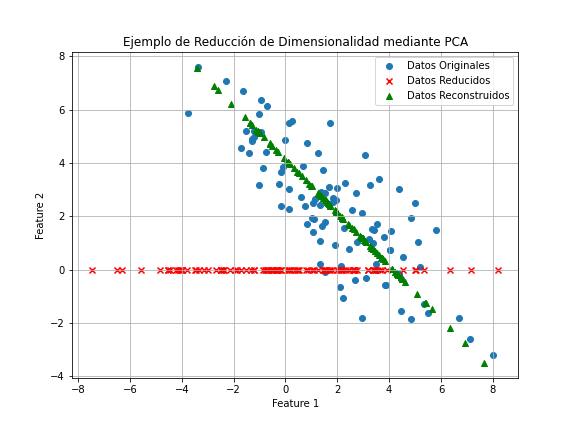
\includegraphics[width=0.7\textwidth]{pca_example.png}
			\caption{Ejemplo de reducción de dimensionalidad mediante PCA.}
		\end{figure}
	\end{frame}
	
	\begin{frame}
		\frametitle{Aplicación en Modelos de Tasas de Interés}
		En finanzas, PCA se utiliza para modelar y analizar curvas de rendimiento de tasas de interés:
		\begin{itemize}
			\item Reduce la complejidad de las curvas.
			\item Captura patrones y tendencias en los movimientos de las tasas.
			\item Ayuda en la gestión de riesgos y toma de decisiones de inversión.
		\end{itemize}
	\end{frame}
	
	\begin{frame}
		\frametitle{Conclusiones}
		\begin{itemize}
			\item PCA es una herramienta poderosa para reducir la dimensionalidad de los datos.
			\item Útil en una amplia gama de campos, incluyendo finanzas.
			\item En modelos de tasas de interés, PCA ayuda a simplificar el análisis y mejora la gestión de riesgos.
		\end{itemize}
	\end{frame}
	
	\begin{frame}
		\frametitle{Referencias}
		\begin{itemize}
			\item Smith, J. Q. (2002). \textit{Using Principal Components to Forecast the Yield Curve}. Journal of Forecasting, 21(5), 393-405.
			\item Jolliffe, I. T. (2002). \textit{Principal Component Analysis}. Wiley Online Library.
		\end{itemize}
	\end{frame}
	
\end{document}
